% answers.tex —— 1977 年·山东A卷 · 参考答案与详细解析片段
% 由 tools/generate_projects.py 依来源总账自 1977/1977_数学真题_山东A_试题.md + 1977/1977_数学真题_山东A_解析正文.md + 1977/1977_数学真题_山东A_答案要点.md 生成，勿手改（改源 MD 后重跑）


\begin{gktip}
固定源是题面与解答连续排印的扫描材料（书籍页码 51—54）。下文逐题对照源解答并重新计算关键结论。三处源卷排印事项在此预告：第 1（2）小题末项「Log 后下标」在扫描件中很小，经高倍局部放大比对，外层下标为封闭双环的「8」、内层下标与相邻全尺寸「3」同形，判定该末项为「底数 8 的对数套底数 3 的对数」，与源解答将其化为「Log₈1」的步骤一致；第 1（5）小题题面「椭园」为「椭圆」之排印变体（保留转录）；第 3 题源解答末行分子印作「Cosx」，系「Cosα」之误排，本文按 $\cos\alpha$ 计算。
\end{gktip}

\begin{answer}
\gksolhead{1}{}

\textbf{题目}：

解下列各题（每小题 5 分）：

（1） $\sqrt{(3-x)^2}=?$

（2） $\lg 2+\lg 5+\lg\sqrt{10}+\lg 0.01+\log_8\log_3 3=?$

（3） 写出函数定义域：

① $y=\log_a x$（$a>0$）；

② $y=\dfrac{\sqrt{x-1}}{x+3}$。

（4） 写出过点 $(2,3)$ 斜率为 $-\dfrac12$ 的直线方程。

（5） 求椭园 $\dfrac{x^2}{25}+\dfrac{y^2}{16}=1$ 的焦点坐标。

\begin{gktip}
\textbf{源注}：原卷印作「椭园」，系「椭圆」之排印变体，本文保留原文字形。
\end{gktip}

（6） 如右图所示的三视图是什么几何体？
\nopagebreak[4]
\begin{center}% 1977 年山东A卷第 1（6）题：正四棱台的三视图——上排为正视图、左视图（两个等腰梯形，带点划线对称轴），下排为俯视图（外大内小两个正方形、四角相连）（按源卷第 2 页布局）
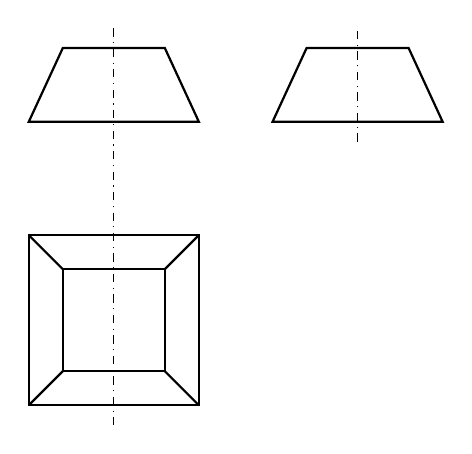
\begin{tikzpicture}[scale=0.72]
  % 正视图（左上）
  \draw[thick] (-1.5,0) -- (1.5,0) -- (0.9,1.3) -- (-0.9,1.3) -- cycle;
  \draw[dashdotted] (0,1.65) -- (0,-5.35);
  % 左视图（右上）
  \begin{scope}[shift={(4.3,0)}]
    \draw[thick] (-1.5,0) -- (1.5,0) -- (0.9,1.3) -- (-0.9,1.3) -- cycle;
    \draw[dashdotted] (0,-0.35) -- (0,1.65);
  \end{scope}
  % 俯视图（左下）
  \draw[thick] (-1.5,-5.0) rectangle (1.5,-2.0);
  \draw[thick] (-0.9,-4.4) rectangle (0.9,-2.6);
  \draw[thick] (-1.5,-2.0) -- (-0.9,-2.6);
  \draw[thick] (1.5,-2.0) -- (0.9,-2.6);
  \draw[thick] (-1.5,-5.0) -- (-0.9,-4.4);
  \draw[thick] (1.5,-5.0) -- (0.9,-4.4);
\end{tikzpicture}
\end{center}
\nopagebreak[4]
\Needspace{4\baselineskip}
\textbf{解析}

\gksubpart{（1）}

\Needspace{5\baselineskip}
由算术平方根的定义，$\sqrt{(3-x)^2}=|3-x|$，按绝对值分段：

\nopagebreak[4]
\[
\sqrt{(3-x)^2}=
\begin{cases}
3-x, & \text{\text{当} } x\le 3 \text{ \text{时}},\\
x-3, & \text{\text{当} } x>3 \text{ \text{时}}.
\end{cases}
\]

（$x=3$ 时两段同为 $0$，分段条件与源解答一致。）

\gksubpart{（2）}

\Needspace{5\baselineskip}
利用 $\lg2+\lg5=\lg10=1$、$\lg\sqrt{10}=\dfrac12\lg10=\dfrac12$、$\lg0.01=-2\lg10=-2$，末项 $\log_3 3=1$、$\log_8 1=0$，故

\nopagebreak[4]
\[
\lg 2+\lg 5+\lg\sqrt{10}+\lg 0.01+\log_8\log_3 3
=1+\frac12-2+0=-\frac12.
\]

\gksubpart{（3）}

① $y=\log_a x$（$a>0$）：真数必须为正，故定义域为 $x>0$。

② $y=\dfrac{\sqrt{x-1}}{x+3}$：被开方式须非负，即 $x\ge1$；此时分母 $x+3>0$ 自然非零。故定义域为 $x\ge1$。

\gksubpart{（4）}

\Needspace{5\baselineskip}
由点斜式，所求直线方程为

\nopagebreak[4]
\[
y-3=-\frac12(x-2),
\qquad\text{\text{即}}\qquad
y=-\frac12x+4.
\]

\gksubpart{（5）}

\Needspace{5\baselineskip}
由 $\dfrac{x^2}{25}+\dfrac{y^2}{16}=1$ 知 $a^2=25$、$b^2=16$，焦点在 $x$ 轴上，故

\nopagebreak[4]
\[
c=\sqrt{a^2-b^2}=\sqrt{5^2-4^2}=3.
\]

焦点坐标为 $F_1(-3,0)$、$F_2(3,0)$。

\gksubpart{（6）}

主视图与左视图都是上下底平行的等腰梯形，俯视图是「外大内小两个正方形、四角对应相连」，即由正方形沿四个角向内收缩形成的台体，对应的几何体是正四棱台。
\nopagebreak[4]
\begin{center}% 1977 年山东A卷第 1（6）题：正四棱台的三视图——上排为正视图、左视图（两个等腰梯形，带点划线对称轴），下排为俯视图（外大内小两个正方形、四角相连）（按源卷第 2 页布局）
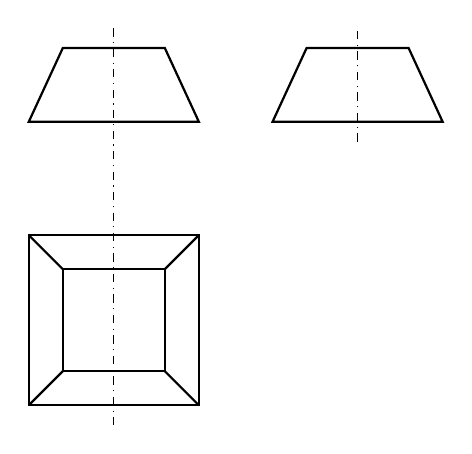
\begin{tikzpicture}[scale=0.72]
  % 正视图（左上）
  \draw[thick] (-1.5,0) -- (1.5,0) -- (0.9,1.3) -- (-0.9,1.3) -- cycle;
  \draw[dashdotted] (0,1.65) -- (0,-5.35);
  % 左视图（右上）
  \begin{scope}[shift={(4.3,0)}]
    \draw[thick] (-1.5,0) -- (1.5,0) -- (0.9,1.3) -- (-0.9,1.3) -- cycle;
    \draw[dashdotted] (0,-0.35) -- (0,1.65);
  \end{scope}
  % 俯视图（左下）
  \draw[thick] (-1.5,-5.0) rectangle (1.5,-2.0);
  \draw[thick] (-0.9,-4.4) rectangle (0.9,-2.6);
  \draw[thick] (-1.5,-2.0) -- (-0.9,-2.6);
  \draw[thick] (1.5,-2.0) -- (0.9,-2.6);
  \draw[thick] (-1.5,-5.0) -- (-0.9,-4.4);
  \draw[thick] (1.5,-5.0) -- (0.9,-4.4);
\end{tikzpicture}
\end{center}
\nopagebreak[4]
\gkanswer{答案（1）：$x\le3$ 时为 $3-x$，$x>3$ 时为 $x-3$。}

\gkanswer{答案（2）：$-\dfrac12$。}

\gkanswer{答案（3）：① $x>0$；② $x\ge1$。}

\gkanswer{答案（4）：$y=-\dfrac12x+4$。}

\gkanswer{答案（5）：$F_1(-3,0)$，$F_2(3,0)$。}

\gkanswer{答案（6）：正四棱台。}

\end{answer}
\begin{answer}
\gksolhead{2}{}

\textbf{题目}（10 分）：

设 $AD$ 是 $\triangle ABC$ 的高，在线段 $BC$ 上取点 $E$，使 $\angle EAC=\angle BAD$，延长 $AE$ 交 $\triangle ABC$ 外接圆于点 $F$。求证：$AF$ 是外接圆的直径。
\nopagebreak[4]
\begin{center}% 1977 年山东A卷第 2 题：三角形 ABC 的外接圆，AD 为高（D 在 BC 上），E 在 BC 上且 A、E、F 共线，F 为 AE 延长线与圆的交点，CF 为虚线辅助线（按源卷第 2 页布局）
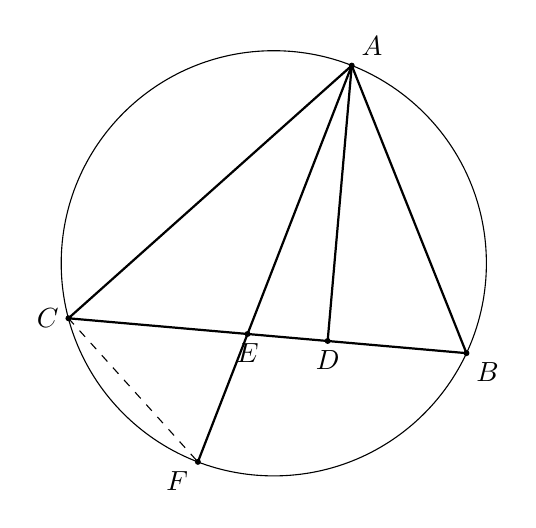
\begin{tikzpicture}[scale=0.9]
  \draw (0,0) circle (3);
  \coordinate (A) at (1.1,2.79);
  \coordinate (B) at (2.719,-1.268);
  \coordinate (C) at (-2.898,-0.776);
  \coordinate (D) at (0.760,-1.096);
  \coordinate (E) at (-0.370,-0.997);
  \coordinate (F) at (-1.071,-2.802);
  \draw[thick] (A) -- (B) -- (C) -- cycle;
  \draw[thick] (A) -- (D);
  \draw[thick] (A) -- (F);
  \draw[dashed] (C) -- (F);
  \fill (A) circle (1.2pt) node[above right] {$A$};
  \fill (B) circle (1.2pt) node[below right] {$B$};
  \fill (C) circle (1.2pt) node[left] {$C$};
  \fill (D) circle (1.2pt) node[below] {$D$};
  \fill (E) circle (1.2pt) node[below] {$E$};
  \fill (F) circle (1.2pt) node[below left] {$F$};
\end{tikzpicture}
\end{center}
\nopagebreak[4]
\Needspace{4\baselineskip}
\textbf{解析}
\nopagebreak[4]
\begin{center}% 1977 年山东A卷第 2 题：三角形 ABC 的外接圆，AD 为高（D 在 BC 上），E 在 BC 上且 A、E、F 共线，F 为 AE 延长线与圆的交点，CF 为虚线辅助线（按源卷第 2 页布局）
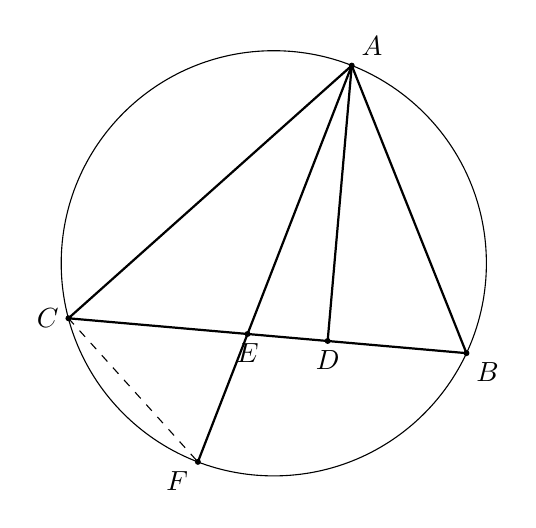
\begin{tikzpicture}[scale=0.9]
  \draw (0,0) circle (3);
  \coordinate (A) at (1.1,2.79);
  \coordinate (B) at (2.719,-1.268);
  \coordinate (C) at (-2.898,-0.776);
  \coordinate (D) at (0.760,-1.096);
  \coordinate (E) at (-0.370,-0.997);
  \coordinate (F) at (-1.071,-2.802);
  \draw[thick] (A) -- (B) -- (C) -- cycle;
  \draw[thick] (A) -- (D);
  \draw[thick] (A) -- (F);
  \draw[dashed] (C) -- (F);
  \fill (A) circle (1.2pt) node[above right] {$A$};
  \fill (B) circle (1.2pt) node[below right] {$B$};
  \fill (C) circle (1.2pt) node[left] {$C$};
  \fill (D) circle (1.2pt) node[below] {$D$};
  \fill (E) circle (1.2pt) node[below] {$E$};
  \fill (F) circle (1.2pt) node[below left] {$F$};
\end{tikzpicture}
\end{center}
\nopagebreak[4]
\Needspace{5\baselineskip}
连接 $FC$。因为 $A$、$E$、$F$ 三点共线（$F$ 在 $AE$ 的延长线上），所以

\nopagebreak[4]
\[
\angle FAC=\angle EAC=\angle BAD.
\]

\Needspace{5\baselineskip}
又在同圆中，$\angle ABC$ 与 $\angle AFC$ 是同弧 $\overset{\frown}{AC}$ 上的圆周角，故

\nopagebreak[4]
\[
\angle ABD=\angle ABC=\angle AFC.
\]

\Needspace{5\baselineskip}
于是在 $\triangle ABD$ 与 $\triangle AFC$ 中有两个角对应相等，两三角形相似，从而第三对角相等：

\nopagebreak[4]
\[
\angle ACF=\angle ADB.
\]

由 $AD$ 是 $\triangle ABC$ 的高，得 $\angle ADB=90^\circ$，所以 $\angle ACF=90^\circ$。而 $\angle ACF$ 是圆上弦 $AF$ 所对的圆周角，其为直角说明 $AF$ 是 $\triangle ABC$ 外接圆的直径。

\gkanswer{答案：见解析版}

\end{answer}
\begin{answer}
\gksolhead{3}{}

\textbf{题目}（15 分）：

$x^2-x\cos\alpha+\dfrac14\sin^2\alpha=0$（$0<\alpha<\dfrac{\pi}{2}$）为关于 $x$ 的二次方程，当 $\alpha$ 为何值时，方程有两个不相等的实数根？它的根是什么？

\Needspace{4\baselineskip}
\textbf{解析}

\Needspace{5\baselineskip}
二次方程的判别式为

\nopagebreak[4]
\[
\Delta=\cos^2\alpha-4\cdot\frac14\sin^2\alpha
=\cos^2\alpha-\sin^2\alpha=\cos2\alpha.
\]

\Needspace{5\baselineskip}
由 $0<\alpha<\dfrac{\pi}{2}$ 得 $0<2\alpha<\pi$。方程有两个不相等的实数根，当且仅当

\nopagebreak[4]
\[
\cos2\alpha>0,
\qquad\text{\text{即}}\qquad
0<2\alpha<\frac{\pi}{2},
\qquad\text{\text{即}}\qquad
0<\alpha<\frac{\pi}{4}.
\]

\Needspace{5\baselineskip}
此时由求根公式，

\nopagebreak[4]
\[
x=\frac{\cos\alpha\pm\sqrt{\cos^2\alpha-\sin^2\alpha}}{2}
=\frac{\cos\alpha\pm\sqrt{\cos2\alpha}}{2}.
\]

\begin{gktip}
\textbf{源注}：源解答末行分子印作「Cosx」，系「Cosα」之误排，本文按 $\cos\alpha$ 转写；判别式条件与根的形式经复算与源解答一致。
\end{gktip}

\gkanswer{答案：当 $0<\alpha<\dfrac{\pi}{4}$ 时，方程有两个不相等的实数根 $x=\dfrac{\cos\alpha\pm\sqrt{\cos2\alpha}}{2}$。}

\end{answer}
\begin{answer}
\gksolhead{4}{}

\textbf{题目}（15 分）：

在半径为 $R$ 的一块圆形铁板上，剪去一个圆心角为 $\alpha$ 弧度的扇形，用剩下的铁板做一个圆锥形容器（铁板厚度和加工量不计）。

（1） 用 $R$ 和 $\alpha$ 表示圆锥底面半径 $r$、圆锥高 $h$、圆锥容积 $V$；

（2） 当 $R=20\,\mathrm{cm}$，$\alpha=\dfrac{2\pi}{5}$ 弧度时，计算圆锥容积 $V$（取 $\pi=3.14$，精确到 $1\,\mathrm{cm^3}$）。

\Needspace{4\baselineskip}
\textbf{解析}

\gksubpart{（1）}

\Needspace{5\baselineskip}
剪去圆心角为 $\alpha$ 的扇形后，剩下扇形的弧长为 $R(2\pi-\alpha)$，它围成圆锥底面圆，故

\nopagebreak[4]
\[
2\pi r=R(2\pi-\alpha),
\qquad
r=\frac{2\pi-\alpha}{2\pi}R.
\]

\Needspace{5\baselineskip}
圆锥的母线长即原圆的半径 $R$，由勾股定理，

\nopagebreak[4]
\[
\begin{aligned}
h&=\sqrt{R^2-r^2}
=R\sqrt{1-\left(\frac{2\pi-\alpha}{2\pi}\right)^2}\\
&=R\sqrt{\frac{4\pi\alpha-\alpha^2}{4\pi^2}}
=\frac{\sqrt{4\pi\alpha-\alpha^2}}{2\pi}R.
\end{aligned}
\]

\Needspace{5\baselineskip}
容积为

\nopagebreak[4]
\[
\begin{aligned}
V&=\frac13\pi r^2h
=\frac13\pi\left(\frac{2\pi-\alpha}{2\pi}R\right)^2\cdot
\frac{\sqrt{4\pi\alpha-\alpha^2}}{2\pi}R\\
&=\frac{R^3(2\pi-\alpha)^2}{24\pi^2}\sqrt{4\pi\alpha-\alpha^2}.
\end{aligned}
\]

\gksubpart{（2）}

\Needspace{5\baselineskip}
当 $R=20\,\mathrm{cm}$、$\alpha=\dfrac{2\pi}{5}$ 时，$2\pi-\alpha=\dfrac{8\pi}{5}$，且

\nopagebreak[4]
\[
4\pi\alpha-\alpha^2
=\frac{2\pi}{5}\left(4\pi-\frac{2\pi}{5}\right)
=\frac{36\pi^2}{25},
\qquad
\sqrt{4\pi\alpha-\alpha^2}=\frac{6\pi}{5}.
\]

\Needspace{5\baselineskip}
代入（1）的结果，

\nopagebreak[4]
\[
\begin{aligned}
V&=\frac{20^3\left(2\pi-\frac{2\pi}{5}\right)^2}{24\pi^2}\cdot
\sqrt{\frac{36\pi^2}{25}}
=\frac{20^3\cdot\frac{64}{25}\pi^2}{24\pi^2}\cdot\frac{6\pi}{5}\\
&=1024\pi.
\end{aligned}
\]

取 $\pi=3.14$，$1024\times3.14=3215.36$，精确到 $1\ \mathrm{cm^3}$，圆锥容积约为 $3215\ \mathrm{cm^3}$。

\gkanswer{答案（1）：$r=\dfrac{2\pi-\alpha}{2\pi}R$，$h=\dfrac{\sqrt{4\pi\alpha-\alpha^2}}{2\pi}R$，$V=\dfrac{R^3(2\pi-\alpha)^2}{24\pi^2}\sqrt{4\pi\alpha-\alpha^2}$。}

\gkanswer{答案（2）：$V=1024\pi\approx3215\ \mathrm{cm^3}$。}

\end{answer}
\begin{answer}
\gksolhead{5}{}

\textbf{题目}（15 分）：

我炮兵阵地位于 $A$，两观察所分别设于 $C$、$D$，已知 $\triangle ACD$ 为一正三角形，且 $CD=a$，当目标出现于 $B$ 时，测得 $\angle CDB=45^\circ$，$\angle BCD=75^\circ$，求炮目距离 $AB$。
\nopagebreak[4]
\begin{center}% 1977 年山东A卷第 5 题：△ACD 为正三角形（CD=a，D 左 C 右），A 为炮兵阵地，B 为目标，四点连成带双对角线的四边形（按源卷第 3 页布局）
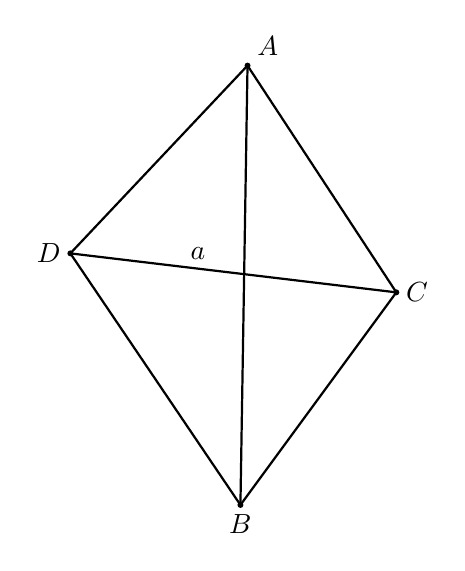
\begin{tikzpicture}[scale=0.9]
  \coordinate (A) at (0.2,3.2);
  \coordinate (D) at (-2.3,0.55);
  \coordinate (C) at (2.3,0);
  \coordinate (B) at (0.1,-3.0);
  \draw[thick] (A) -- (D) -- (C) -- cycle;
  \draw[thick] (A) -- (B);
  \draw[thick] (D) -- (B);
  \draw[thick] (C) -- (B);
  \fill (A) circle (1.2pt) node[above right] {$A$};
  \fill (D) circle (1.2pt) node[left] {$D$};
  \fill (C) circle (1.2pt) node[right] {$C$};
  \fill (B) circle (1.2pt) node[below] {$B$};
  \node at (-0.5,0.55) {$a$};
\end{tikzpicture}
\end{center}
\nopagebreak[4]
\Needspace{4\baselineskip}
\textbf{解析}
\nopagebreak[4]
\begin{center}% 1977 年山东A卷第 5 题：△ACD 为正三角形（CD=a，D 左 C 右），A 为炮兵阵地，B 为目标，四点连成带双对角线的四边形（按源卷第 3 页布局）
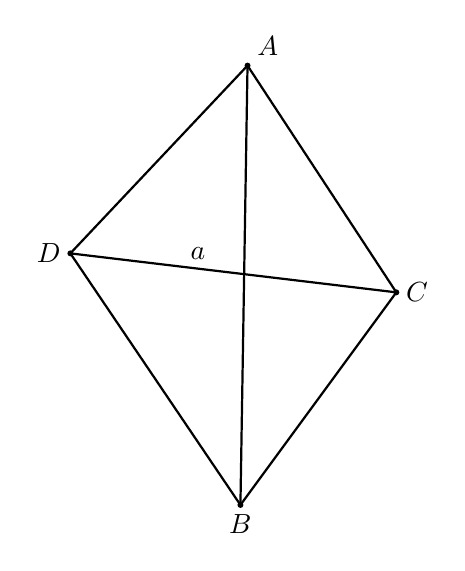
\begin{tikzpicture}[scale=0.9]
  \coordinate (A) at (0.2,3.2);
  \coordinate (D) at (-2.3,0.55);
  \coordinate (C) at (2.3,0);
  \coordinate (B) at (0.1,-3.0);
  \draw[thick] (A) -- (D) -- (C) -- cycle;
  \draw[thick] (A) -- (B);
  \draw[thick] (D) -- (B);
  \draw[thick] (C) -- (B);
  \fill (A) circle (1.2pt) node[above right] {$A$};
  \fill (D) circle (1.2pt) node[left] {$D$};
  \fill (C) circle (1.2pt) node[right] {$C$};
  \fill (B) circle (1.2pt) node[below] {$B$};
  \node at (-0.5,0.55) {$a$};
\end{tikzpicture}
\end{center}
\nopagebreak[4]
\Needspace{5\baselineskip}
在 $\triangle BCD$ 中，$\angle CBD=180^\circ-(45^\circ+75^\circ)=60^\circ$。由正弦定理，

\nopagebreak[4]
\[
BC=\frac{a\sin45^\circ}{\sin60^\circ}
=a\cdot\frac{\dfrac{\sqrt2}{2}}{\dfrac{\sqrt3}{2}}
=\frac{\sqrt6}{3}\,a.
\]

\Needspace{5\baselineskip}
又 $\angle ACB=\angle ACD+\angle DCB=60^\circ+75^\circ=135^\circ$，$AC=a$（正三角形边长）。在 $\triangle ABC$ 中由余弦定理，

\nopagebreak[4]
\[
\begin{aligned}
AB^2&=AC^2+BC^2-2\cdot AC\cdot BC\cdot\cos\angle ACB\\
&=a^2+\frac23a^2-2a\cdot\frac{\sqrt6}{3}\,a\cos(75^\circ+60^\circ)\\
&=\frac53a^2+\frac{2\sqrt6}{3}\,a^2\cos45^\circ
=\frac53a^2+\frac{2\sqrt6}{3}\,a^2\cdot\frac{\sqrt2}{2}\\
&=\frac{5+2\sqrt3}{3}\,a^2.
\end{aligned}
\]

\Needspace{5\baselineskip}
所以

\nopagebreak[4]
\[
AB=\sqrt{\frac{5+2\sqrt3}{3}}\,a
=\frac{\sqrt{15+6\sqrt3}}{3}\,a.
\]

\gkanswer{答案：$AB=\dfrac{\sqrt{15+6\sqrt3}}{3}\,a$。}

\end{answer}
\begin{answer}
\gksolhead{6}{}

\textbf{题目}（15 分）：

现有可建猪圈 $L$ 米的材料，要建彼此相连的 $m$ 间面积相等的矩形猪圈（如下图）（门在内，墙的厚度不计）。怎样设计每间猪圈的长和宽，才能使所建的猪圈的总面积最大？按这种设计，$m$ 间猪圈长的总和与宽的总和有什么关系？
\nopagebreak[4]
\begin{center}% 1977 年山东A卷第 6 题：m 间彼此相连的矩形猪圈——整排总长 x 标在上方，每间宽 (L-2x)/(m+1) 标在右侧，下方横线与「m 间」表示整排共 m 间（按源卷第 4 页布局）
\begin{tikzpicture}[scale=0.85]
  \draw[thick] (0,0) rectangle (8,2.4);
  \draw[thick] (1.0,0) -- (1.0,2.4);
  \draw[thick] (2.0,0) -- (2.0,2.4);
  \draw[thick] (3.0,0) -- (3.0,2.4);
  \draw[thick] (4.0,0) -- (4.0,2.4);
  \draw[thick] (6.8,0) -- (6.8,2.4);
  \node at (5.4,1.2) {$\cdots$};
  \node[above] at (4.0,2.55) {$x$};
  \node[right] at (8.2,1.2) {$\dfrac{L-2x}{m+1}$};
  \draw[thick] (0,-0.55) -- (8,-0.55);
  \draw[thick] (0,-0.38) -- (0,-0.72);
  \draw[thick] (8,-0.38) -- (8,-0.72);
  \node[below] at (4.0,-0.78) {$m$ 间};
\end{tikzpicture}
\end{center}
\nopagebreak[4]
\begin{gktip}
\textbf{参考题}（不作录取成绩，考生可视能力尽量作）
\end{gktip}

\Needspace{5\baselineskip}
\textbf{参考题 1．} 求极限：

\nopagebreak[4]
\[
\lim_{x\to\infty}\frac{\mathrm e^x}{x^2}.
\]

\textbf{参考题 2．} 利用定积分证明：椭圆 $\dfrac{x^2}{a^2}+\dfrac{y^2}{b^2}=1$ 的面积 $S=\pi ab$。

\Needspace{4\baselineskip}
\textbf{解析}
\nopagebreak[4]
\begin{center}% 1977 年山东A卷第 6 题：m 间彼此相连的矩形猪圈——整排总长 x 标在上方，每间宽 (L-2x)/(m+1) 标在右侧，下方横线与「m 间」表示整排共 m 间（按源卷第 4 页布局）
\begin{tikzpicture}[scale=0.85]
  \draw[thick] (0,0) rectangle (8,2.4);
  \draw[thick] (1.0,0) -- (1.0,2.4);
  \draw[thick] (2.0,0) -- (2.0,2.4);
  \draw[thick] (3.0,0) -- (3.0,2.4);
  \draw[thick] (4.0,0) -- (4.0,2.4);
  \draw[thick] (6.8,0) -- (6.8,2.4);
  \node at (5.4,1.2) {$\cdots$};
  \node[above] at (4.0,2.55) {$x$};
  \node[right] at (8.2,1.2) {$\dfrac{L-2x}{m+1}$};
  \draw[thick] (0,-0.55) -- (8,-0.55);
  \draw[thick] (0,-0.38) -- (0,-0.72);
  \draw[thick] (8,-0.38) -- (8,-0.72);
  \node[below] at (4.0,-0.78) {$m$ 间};
\end{tikzpicture}
\end{center}
\nopagebreak[4]
\Needspace{5\baselineskip}
设整排的总长为 $x$ 米，每间宽为 $w$ 米。材料由上下两排长 $2x$ 与 $m+1$ 道宽 $w$（两端与 $m-1$ 道隔墙）组成，故 $2x+(m+1)w=L$，即

\nopagebreak[4]
\[
w=\frac{L-2x}{m+1}.
\]

\Needspace{5\baselineskip}
每间长为 $\dfrac{x}{m}$，$m$ 间总面积为

\nopagebreak[4]
\[
S=x\cdot\frac{L-2x}{m+1}
=-\frac{2}{m+1}x^2+\frac{L}{m+1}x.
\]

\Needspace{5\baselineskip}
这是 $x$ 的二次函数，其中 $a=-\dfrac{2}{m+1}<0$、$b=\dfrac{L}{m+1}$，故当

\nopagebreak[4]
\[
x=-\frac{b}{2a}=\frac{\dfrac{L}{m+1}}{\dfrac{4}{m+1}}=\frac{L}{4}
\]

\Needspace{5\baselineskip}
时，面积 $S$ 最大，其值

\nopagebreak[4]
\[
S_{\max}=\frac{L}{4}\cdot\frac{L-\frac{L}{2}}{m+1}
=\frac{L^2}{8(m+1)}.
\]

\Needspace{5\baselineskip}
这时每间的宽与长分别为

\nopagebreak[4]
\[
\frac{L-2x}{m+1}=\frac{L}{2(m+1)},
\qquad
\frac{x}{m}=\frac{L}{4m}.
\]

此时猪圈长的总和为 $2x=\dfrac{L}{2}$，宽的总和为 $(m+1)\cdot\dfrac{L}{2(m+1)}=\dfrac{L}{2}$，两者相等。

\textbf{参考题 1}

\Needspace{5\baselineskip}
由 $\dfrac{\mathrm e^x}{x^2}$ 在 $x\to\infty$ 时为 $\dfrac{\infty}{\infty}$ 型，两次用洛必达法则，

\nopagebreak[4]
\[
\lim_{x\to\infty}\frac{\mathrm e^x}{x^2}
=\lim_{x\to\infty}\frac{\mathrm e^x}{2x}
=\lim_{x\to\infty}\frac{\mathrm e^x}{2}=+\infty,
\]

即该极限不存在有限的极限值，与源解答结论「极限不存在」一致（当 $x\to\infty$ 时函数趋于 $+\infty$）。

\textbf{参考题 2}

\Needspace{5\baselineskip}
先求椭圆在第一象限内的面积 $S'$：

\nopagebreak[4]
\[
S'=\int_0^a b\sqrt{1-\frac{x^2}{a^2}}\,dx
=\frac ba\int_0^a\sqrt{a^2-x^2}\,dx.
\]

\Needspace{5\baselineskip}
令 $x=a\sin t$，则 $\sqrt{a^2-x^2}=a\cos t$，$dx=a\cos t\,dt$（$0\le t\le\dfrac{\pi}{2}$），

\nopagebreak[4]
\[
\begin{aligned}
S'&=\frac ba\int_0^{\frac{\pi}{2}}a\cos t\cdot a\cos t\,dt
=ab\int_0^{\frac{\pi}{2}}\cos^2t\,dt\\
&=ab\int_0^{\frac{\pi}{2}}\frac{\cos2t+1}{2}\,dt
=ab\left(\frac{\sin2t}{4}+\frac t2\right)\Bigg|_0^{\frac{\pi}{2}}
=\frac{ab\pi}{4}.
\end{aligned}
\]

\Needspace{5\baselineskip}
由对称性，椭圆的面积

\nopagebreak[4]
\[
S=4S'=\pi ab.
\]

\gkanswer{答案：每间长 $\dfrac{L}{4m}$、宽 $\dfrac{L}{2(m+1)}$ 时总面积最大，最大面积为 $\dfrac{L^2}{8(m+1)}$；此时 $m$ 间猪圈长的总和与宽的总和相等，均为 $\dfrac{L}{2}$。}

\end{answer}